\documentclass[border=6pt]{standalone}
\usepackage{tikz}
\usetikzlibrary{arrows.meta,calc,decorations.pathreplacing}
\begin{document}
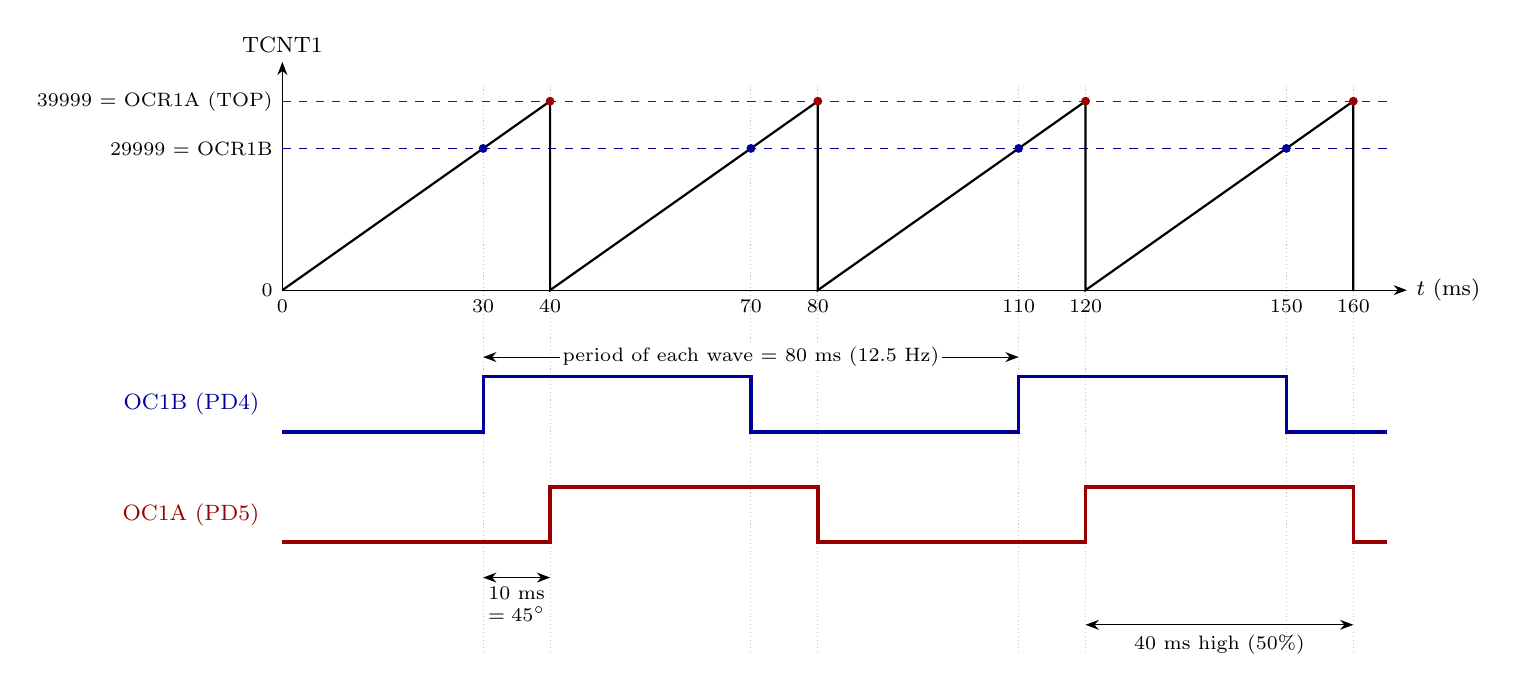
\begin{tikzpicture}[>=Stealth,font=\small,x=0.085cm,y=1cm]
% time axis: 1 unit = 1 ms (1 tick = 1 us, 40000 ticks = 40 ms per ramp)
\def\H{2.4}% height of TOP = 39999
% grid
\foreach \t in {30,40,70,80,110,120,150,160} \draw[gray!45,densely dotted] (\t,-4.6) -- (\t,\H+0.2);
% TCNT1 axes
\draw[->] (0,0) -- (0,\H+0.5) node[above,font=\footnotesize]{TCNT1};
\draw[->] (0,0) -- (168,0) node[right,font=\footnotesize]{$t$ (ms)};
\node[anchor=east,font=\scriptsize] at (0,\H) {39999 = OCR1A (TOP)};
\node[anchor=east,font=\scriptsize] at (0,0.75*\H) {29999 = OCR1B};
\node[anchor=east,font=\scriptsize] at (0,0) {0};
\draw[blue!60!black,dashed] (0,0.75*\H) -- (165,0.75*\H);
\draw[red!60!black,dashed] (0,\H) -- (165,\H);
\draw[thick] (0,0) \foreach \k in {0,1,2,3} { -- (40*\k+40,\H) -- (40*\k+40,0) };
\foreach \k in {0,1,2,3} {
  \fill[blue!60!black] (40*\k+30,0.75*\H) circle (1.6pt);
  \fill[red!60!black] (40*\k+40,\H) circle (1.6pt);
}
\foreach \t in {0,30,40,70,80,110,120,150,160} \node[below,font=\scriptsize] at (\t,0) {\t};
% OC1B
\begin{scope}[yshift=-1.8cm]
\node[anchor=east,font=\footnotesize,blue!60!black] at (-2,0.35) {OC1B (PD4)};
\draw[very thick,blue!60!black] (0,0) -- (30,0) -- (30,0.7) -- (70,0.7) -- (70,0) -- (110,0) -- (110,0.7) -- (150,0.7) -- (150,0) -- (165,0);
\end{scope}
% OC1A
\begin{scope}[yshift=-3.2cm]
\node[anchor=east,font=\footnotesize,red!60!black] at (-2,0.35) {OC1A (PD5)};
\draw[very thick,red!60!black] (0,0) -- (40,0) -- (40,0.7) -- (80,0.7) -- (80,0) -- (120,0) -- (120,0.7) -- (160,0.7) -- (160,0) -- (165,0);
\end{scope}
% annotations
\draw[<->] (30,-3.65) -- (40,-3.65) node[midway,below,font=\scriptsize,align=center]{10 ms\\$=45^\circ$};
\draw[<->] (30,-0.85) -- (110,-0.85) node[pos=0.5,fill=white,font=\scriptsize,inner sep=1pt]{period of each wave = 80 ms (12.5 Hz)};
\draw[<->] (120,-4.25) -- (160,-4.25) node[midway,below,font=\scriptsize]{40 ms high (50\%)};
\end{tikzpicture}
\end{document}
